\chapter{变分法}\label{variant-of-calculus}

\section{变分法原理}
\subsection{变分的定义}
\subsubsection{积分的变分}
\paragraph*{一元积分}$x$为自变量,$y(x)$为一个光滑函数,取$\varepsilon$为一极小量,$\eta(x)$为一光滑函数。积分
$$I(y)=\int_a^b F(x,y(x),y'(x))\dif x$$
则定义
\begin{empheq}{align}
I(y+\delta\eta)-I(y)&=\int_a^b F(x,y+\delta\eta,(y+\delta\eta)')-F(x,y,y')\dif x\\
&=\int_a^b \left[\left(\delta y\pdv{}{y}+(\delta y)'\pdv{}{y'}\right)F+\inv{2}\left(\delta y\pdv{}{y}+(\delta y)'\pdv{}{y'}\right)^2F+\cdots\right]\dif x\\
&=\delta I(y)+\inv{2}\delta^2I(y)+\cdots
\end{empheq}

于是可以看出:
\begin{empheq}{align}
\delta I(y)&=\int_a^b \left(\delta y\pdv{}{y}+(\delta y)'\pdv{}{y'}\right)F\dif x\\
&=\int_a^b \delta y\pdv{F}{y}\dif x+\left.\delta y\pdv{F}{y'}\right|_a^b-\int_a^b \delta y\odv{}{x}\pdv{F}{y}\dif x\\
&=\int_a^b \left(\pdv{F}{y}-\odv{}{x}\pdv{F}{y'}\right)\delta y\dif x
\end{empheq}
这里用了分部积分。

从以上可以看出,所谓变分,就是在一个光滑函数的微小扰动下积分的改变量。

\paragraph*{一阶最优条件}问题
$$\min_y I(y)$$
的一阶条件就是
\begin{empheq}{equation}\label{1d-varition-min-1st-order-cond}
\delta I(y)=0\implies \pdv{F}{y}-\odv{}{x}\pdv{F}{y'}=0
\end{empheq}

有的地方也这样定义变分:
\begin{empheq}{align}
\delta_1 I(y,\eta)&=\left.\odv{I(y+\varepsilon \eta)}{\varepsilon}\right|_{\varepsilon=0}\\
&=\int_a^b \left(\pdv{F}{y}-\odv{}{x}\pdv{F}{y'}\right)\dif x\\
&=\frac{\delta I}{\delta}
\end{empheq}
这个定义与前面的实质相同。叫做Gateaux变分,是方向导数的推广。物理学中前一种用的多,Gateaux用的不多。

\paragraph*{一阶最优条件的特殊情形}

\begin{description}
\item[不显含$x$] 函数为$F(y,y')$。取
\begin{empheq}{align}
\odv{}{x}\left(y'\pdv{F}{y'}-F\right)&=y''\pdv{F}{y'}+y'\odv{}{x}\pdv{F}{y'}-\left(\pdv{F}{y}y'+\pdv{F}{y'}y''\right)\\
&=-y'\left(\pdv{F}{y}-\odv{}{x}\pdv{F}{y'}\right)\\
\implies &F-y'\pdv{F}{y'}=\text{const} \label{1d-varition-min-1st-order-cond-special-1}
\end{empheq}
\item[不显含$y$] 函数为$F(x,y')$,直接代入有:
\begin{empheq}{equation}\label{1d-varition-min-1st-order-cond-special-2}
\pdv{F}{y'}=\text{const}
\end{empheq}
\item[不显含$y'$] 函数为$F(x,y)$。 直接代入\cref{1d-varition-min-1st-order-cond}即得:
\begin{empheq}{equation}\label{1d-varition-min-1st-order-cond-special-3}
\pdv{F}{y}=0
\end{empheq}

\end{description}

\paragraph*{一元变分与偏微分记号}假如$F$函数不显含$y'$,则有
\begin{empheq}{align}
\delta I=\int_a^b \varepsilon y\pdv{F}{y}\dif x
\end{empheq}
则可以记
$$\frac{\delta I}{\varepsilon y}=\pdv{I}{y}=\pdv{F}{y}$$
一阶条件\cref{1d-varition-min-1st-order-cond}现在就是
$$\pdv{F}{y}=0$$
这里的偏微分只是一种记号,不要把它与一般的微分混淆。$\pdv{F}{y}$是$x$的函数,但是$I$本身是一个积分,不是$x$的函数。
\paragraph*{多元积分}考虑一个更一般的多元积分:
$$I(y)=\int_{\Omega}F(\bx, y(\bx),\nabla y(\bx))\dif V$$
$\bx\in\Rns$,$y$仍是标量函数,此时
\begin{empheq}{align}
\delta I(y)&=\int_{\Omega} \left(\pdv{L}{y}-\sum_k \pdv{}{x_k}\pdv{F}{y_k'}\right)\delta y\dif V
\end{empheq}
这里$u_k'=\pdv{y}{x_k}$。
\subsubsection{变分运算的法则}
\begin{enumerate}
\item 与微分交换:
$$(\delta y)'=\delta y'$$
\item 与积分交换:
$$\delta \int_a^b F\dif x=\int_a^b \delta F\dif x$$
\item 复合函数的变分与微分相同:
$$\delta F(x,y,y')=F_2\delta y+F_3\delta y'$$
\end{enumerate}
\subsection{约束变分与拉格朗日法}

\section{变分法的应用}

\subsection{几何优化}

\subsection{运动学}
\subsubsection{最速降线}
\paragraph*{曲线方程}
\begin{example}
建立如下坐标系:
\begin{center}
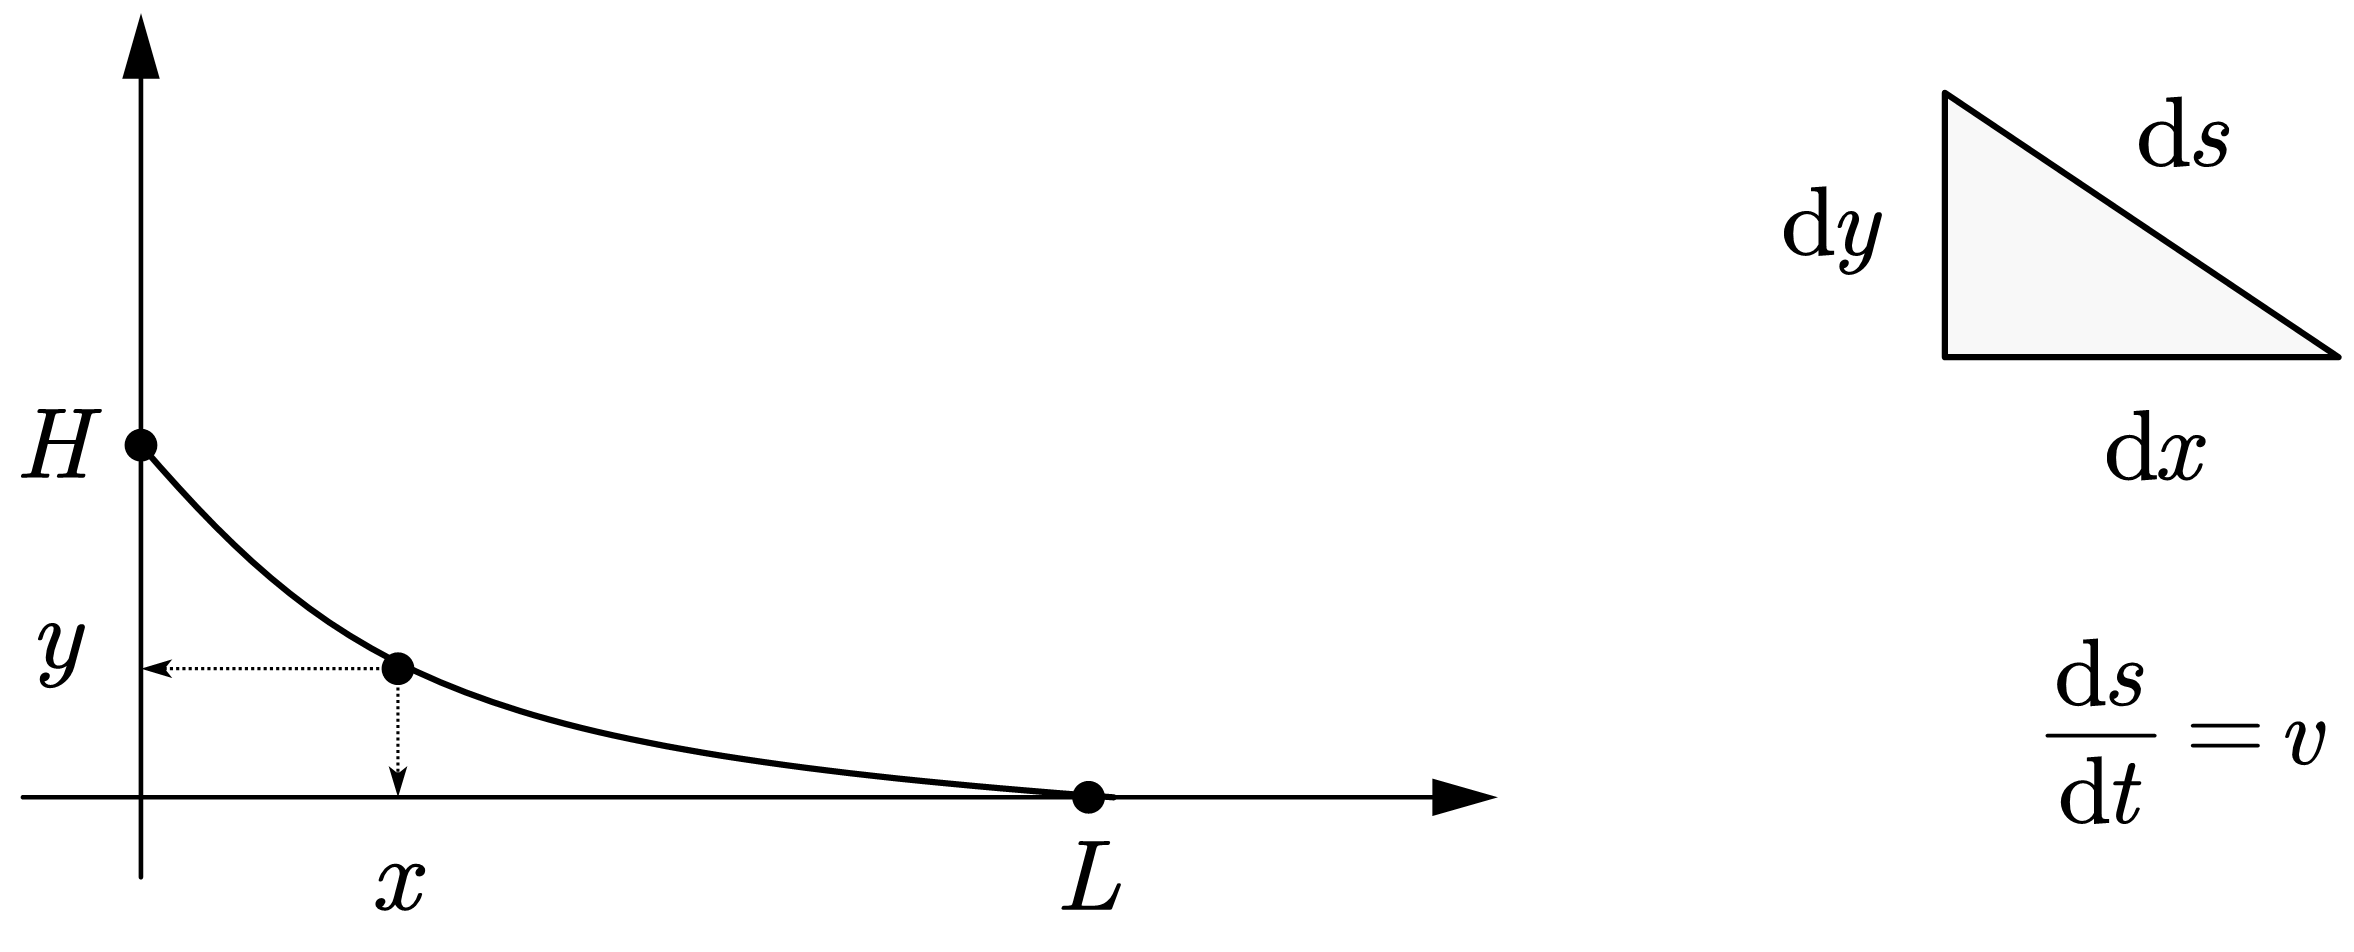
\includegraphics[width=8cm]{figure/fastest-path.png}
\end{center}
求最速降线方程,这条线也叫Brachistochrone curve。需要强调,图中只是一种示意,不代表路径必然在$x$轴上方,有可能某一部分是在下方的。
\end{example}
\begin{solution}
我们的求解目标是:
$$\min \int_0^T\dif t,\quad y(x=0)=H,y(x=L)=0$$
但积分是要对$x$进行的,因此需要得到$\dif t,\dif x$的关系式。如示意图所示,根据能量守恒有:
\begin{empheq}{equation}\label{fastest-desc-path-dx-dt}
\odv{s}{t}=v=\sqrt{2g(H-y)}=\frac{\dif x\sqrt{1+(y')^2}}{t}\ \implies \ \dif t=\sqrt{\frac{1+(y')^2}{2g(H-y)}}\dif x
\end{empheq}

于是现在的优化目标是:
\begin{empheq}{equation}\label{fastest-desc-path-target-transform}
\min_y\quad \int_0^L\sqrt{\frac{1+(y')^2}{2g(H-y)}}\dif x
\end{empheq}

可以忽略常数$g$。根据不显含$x$的特殊一阶条件\cref{1d-varition-min-1st-order-cond-special-1},可得:
$$\sqrt{\frac{1+(y')^2}{(H-y)}}-\frac{1}{\sqrt{(1+(y')^2)(H-y)}}(y')^2=C$$
左边为
$$\inv{\sqrt{H-y}}\inv{\sqrt{1+(y')^2}}>0$$
因此$C>0$。上式还可转化为:
\begin{empheq}{equation}\label{fastest-path-cond-deriv}
1+(y')^2=\inv{C^2}\inv{(H-y)}
\end{empheq}
由于$1+(y')^2\geq1$,因此$C^2(H-y)\leq 1$。

解上式时,可以直接解出$y'$,再解微分方程。另一种技巧是换元
\begin{empheq}{equation}\label{fastest-desc-path-target(theta)}
H-y=\inv{C^2}\sin^2\theta\implies 1+(y')^2=\inv{\sin^2\theta},\frac{1+(y')^2}{H-y}=\frac{C^2}{\sin^4\theta}
\end{empheq}
不妨取$\theta\geq 0$。同时根据上式有
\begin{empheq}{equation}\label{fastest-desc-path-target(theta)}
y'=-\inv{C^2}\sin(2\theta)\theta'
\end{empheq}
代入式\cref{fastest-desc-path-target(theta)},即有:
\begin{empheq}{equation}\label{fastest-desc-path-dtheta-dx}
\odv{\theta}{x}=\theta'=\pm\frac{C^2}{2\sin^2\theta}
\end{empheq}
可以解出
\begin{empheq}{equation}\label{fastest-desc-path-x-theta}
C^2x+C_1=\pm\left(\theta-\inv{2}\sin(2\theta)\right)
\end{empheq}

现在考虑定解条件:$x=0, y=H\implies\theta=0\implies C_1=0$。当$x=L$时,$y=0,H=\inv{C^2}\sin^2(\theta),C^2L=\pm\left(\theta-\inv{2}\sin(2\theta)\right)$。

分开考虑,$L>0$时,$4C^2L>0$,取$4C^2L=\theta-\inv{2}\sin(2\theta)$,结合$HC^2=\sin^2\theta$,有:
\begin{empheq}{equation}\label{fastest-desc-path-theta-max}
\frac{L}{H}=\frac{\theta-\inv{2}\sin(2\theta)}{\sin^2\theta}
\end{empheq}
据此可以解出$\theta_{\max}$,同时得到
\begin{empheq}{equation}\label{fastest-desc-path-C}
C=\sqrt{\frac{\sin^2\theta_{\max}}{H}}
\end{empheq}
则可以得参数方程形式的解:
\begin{empheq}[left=\empheqlbrace]{align}
x(\theta)&=\frac{1}{C^2}(\theta-\inv{2}\sin(2\theta))\\
y(\theta)&=H-\frac{\sin^2\theta}{C^2}\\
\theta&\in[0,\theta_{\max}]
\end{empheq}
当$L<0$时,$x$取反即可。或者让$x$乘上一个因子$\sign(L)$。这里需要注意,$x$是$\theta$的单调函数,但$y$不是。根据这个解,可以直接得到$\dot{x}(0)=0,\dot{y}(0)=0$。

能否根据$\sin\theta=\sqrt{C^2(H-y)},\theta=\arcsin \sqrt{C^2(H-y)}$代入$2C^2L$的等式解出$C$呢?这不太容易,因为一般来说$\arcsin\in\left[-\frac{\pi}{2},\frac{\pi}{2}\right]$,但本例中$\theta$是可以大于$\hpi$的,于是不一定能解出$C$。 

这是说周期函数的反函数不是单值函数,最好不要用。

\end{solution}

\paragraph*{坐标-时间}现在考虑运动时间。根据解可直接得到:
\begin{empheq}[left=\empheqlbrace]{align}\label{fastest-desc-path-xy-dot}
\dot{x}&=\frac{2\sin^2\theta}{C^2}\dot{\theta}\\
\dot{y}&=-\frac{\sin(2\theta)}{C^2}\dot{\theta}
\end{empheq}

需要求出$\dot{\theta}$。不妨假定$L>0$。则由\cref{fastest-desc-path-dtheta-dx}得到:
\begin{empheq}{equation}
\dif x=\frac{2\sin^2\theta}{C^2}\dif \theta
\end{empheq}

再根据式\cref{fastest-desc-path-target(theta)}给出的被积函数与$\theta$的关系式,可知:
\begin{empheq}{align}
t(x)&=\int_0^x \sqrt{\frac{1+(y')^2}{2g(H-y)}}\dif x\\
&=\int_0^{x^{-1}(x)}\inv{\sqrt{2g}} \frac{C}{\sin^2\theta}\frac{2\sin^2\theta}{C^2}\dif \theta\\
&=\frac{2}{\sqrt{2g}C}x^{-1}(x)
\end{empheq}
这里给出了时间与$x$坐标的关系。反之,$\theta$与$t$的关系就是:
\begin{empheq}{equation}
x(t)=x\left(\frac{\sqrt{2g}C}{2}t\right)\implies
\theta(t)=\frac{\sqrt{2g}C}{2}t
\end{empheq}
顺便也得到了$y(t)$。

最长运动时间
\begin{empheq}{equation}
t_{\max}=\frac{2}{\sqrt{2g}C}\theta_{\max}
\end{empheq}

\paragraph*{验证能量守恒}
现在验证此时$\sqrt{(\dot{x})^2+(\dot{y})^2}\stackrel{?}{=}\sqrt{2g(H-y)}$,即由能量守恒给出的速度是否与运动方程给出的相同。
\begin{empheq}{align}
\sqrt{(\dot{x})^2+(\dot{y})^2}&=\sqrt{\left(\frac{2\sin^2\theta}{C^2}\right)^2+\left(-\frac{\sin(2\theta)}{C^2}\right)^2}\frac{\sqrt{2g}C}{2}\\
&=\sqrt{2g}\frac{\sin\theta}{C}\\
\sqrt{2g(H-y)}&=\sqrt{2g}\sqrt{\frac{\sin^2\theta}{C^2}}\\
&=\sqrt{2g}\frac{\sin\theta}{C}
\end{empheq}
两式相等,能量守恒成立。

\paragraph*{特殊情况}现在来考虑一个问题,给定$H$,假如我们希望到达底部时,$\dot{y}=0$,也就是速度平行于$x$轴,则$L$应当怎么取?

根据式\cref{fastest-desc-path-xy-dot}有:
\begin{empheq}{equation}
\dot{y}=-\inv{C^2}\sin(2\theta)\dot{\theta}=0
\end{empheq}
由于$\dot{\theta}>0$,因此必有$\theta_{\max}=\hpi$。回代到\cref{fastest-desc-path-theta-max,fastest-desc-path-C},即有:
\begin{empheq}{align}
\frac{L}{H}&=\frac{\pi}{2}\\
C&=\inv{\sqrt{H}}
\end{empheq}

\paragraph*{数值解}
\begin{center}
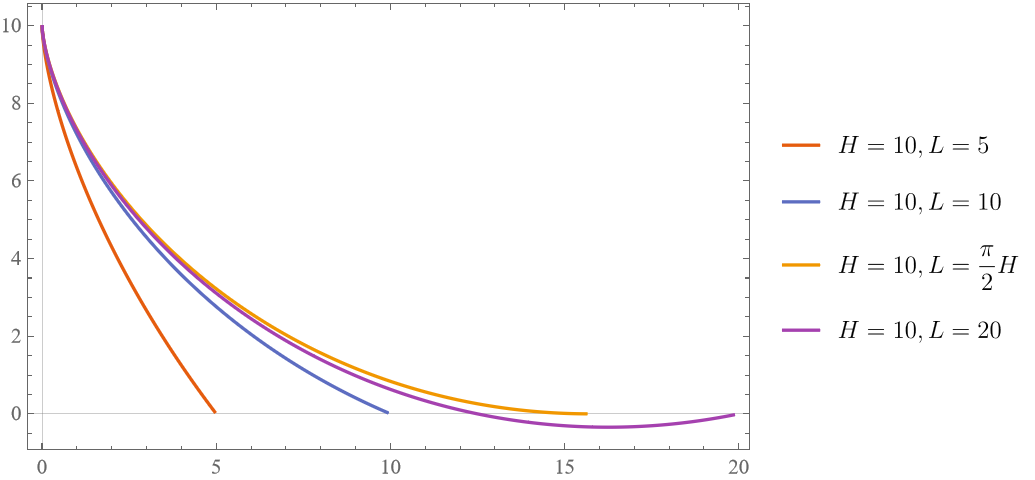
\includegraphics[width=10cm]{figure/fastest-descedning.png}
\end{center}

\subsubsection{最速升线}
\paragraph*{无约束}
\begin{example}
有最速降线,就有最速升线。如图所示:
\begin{center}
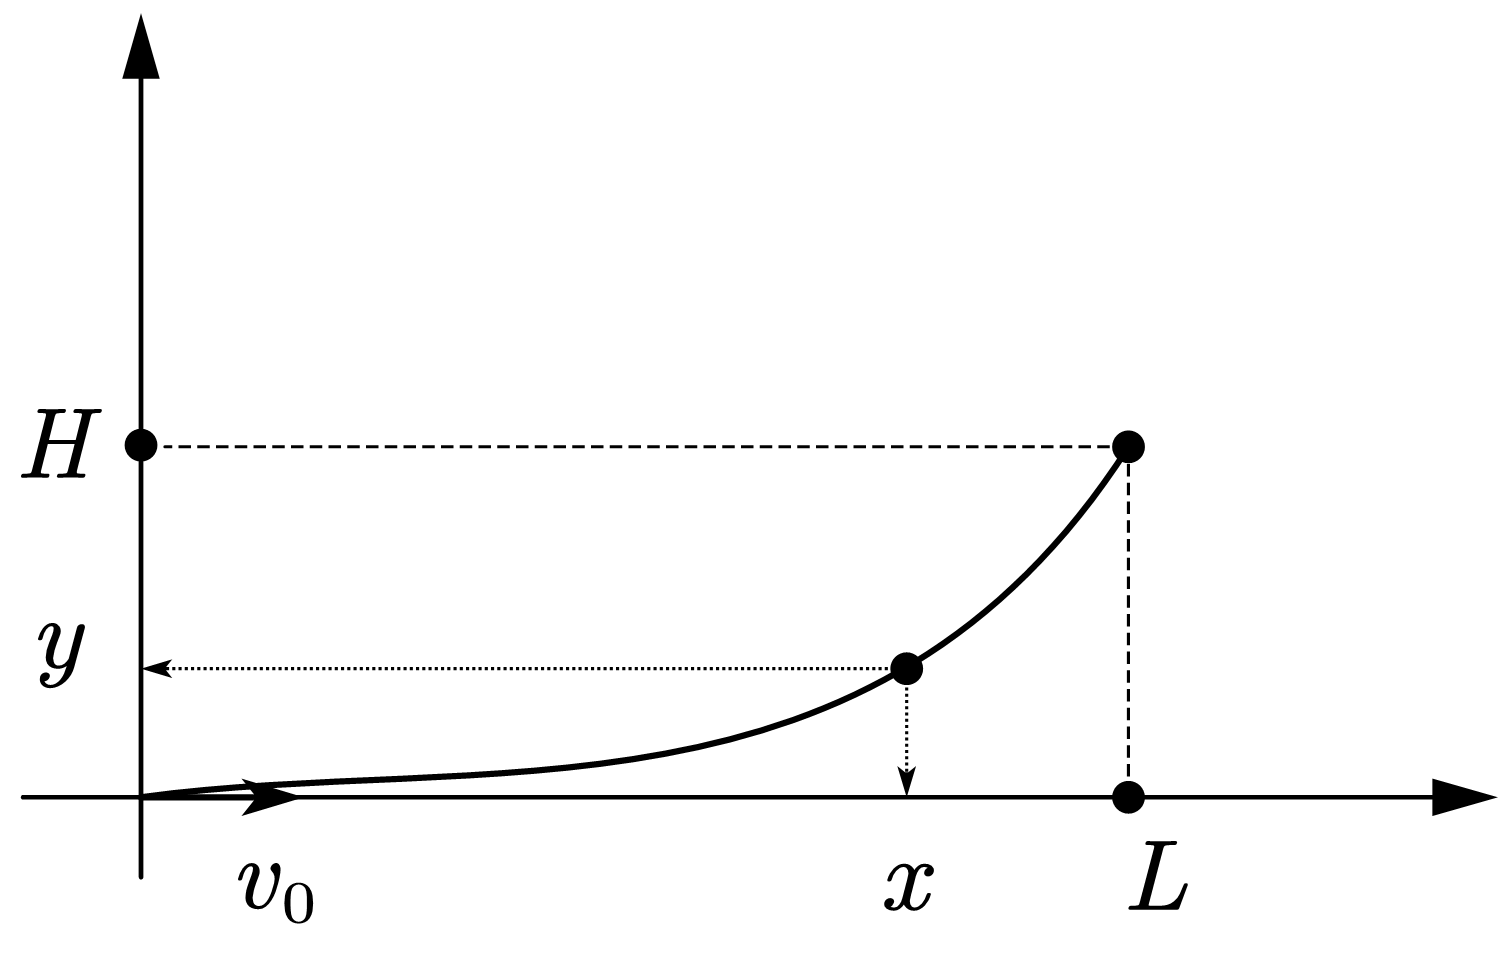
\includegraphics[width=6cm]{figure/fastest-ascending.png}
\end{center}
假定初始速度$v_0$,出发点为原点。显然,边界条件为$y(x=0)=0,y(x=L)=H$。
\end{example}
\begin{solution}
仍然沿用之前的做法,只是根据能量守恒,现在
$$v=\sqrt{2g\left(\frac{v_0^2}{2g}-y\right)}$$
$H$满足的限制为:
$$H\leq\frac{v_0^2}{2g}$$
对比最速降线中的速度\cref{fastest-desc-path-dx-dt},可知,现在的被积函数只是把$H$换成$\frac{v_0^2}{2g}$,此外边界条件有所改变,因此最后得到的是最速降线的一个镜像对称。

直到最速降线的\cref{fastest-desc-path-x-theta}的推导都是相同的,只是把被积表达式中的$H$换成$\frac{v_0^2}{2g}$。关键结论如下:
\begin{empheq}{align}
\frac{v_0^2}{2g}-y&=\frac{\sin^2\theta}{C^2}\implies 1+(y')^2=\inv{\sin^2\theta},\frac{1+(y')^2}{\frac{v_0^2}{2g}-y}=\frac{C^2}{\sin^4\theta}\label{fastest-asc-transform}\\
C^2x+C_1&=\pm\left(\theta-\inv{2}\sin(2\theta)\right)\label{fastest-asc-x-eq}
\end{empheq}

直接考虑定解条件。由两个边界条件代入换元表达式\cref{fastest-asc-transform}有:
\begin{empheq}{align}
\frac{v_0^2}{2g}&=\frac{\sin^2\theta_0}{C^2}\\
\frac{v_0^2}{2g}-H&=\frac{\sin^2\theta_1}{C^2}
\end{empheq}
易知$\sin^2\theta_1<\sin^2\theta_0$,由于$\theta>0$,因此$\theta_1<\theta_0$。再把两个边界条件代入\cref{fastest-asc-x-eq},有:
\begin{empheq}{align}
C_1&=\pm\left(\theta_0-\inv{2}\sin(2\theta_0)\right)\\
C^2L+C_1&=\pm\left(\theta_1-\inv{2}\sin(2\theta_1)\right)
\end{empheq}
未知数为$\theta_0,\theta_1,C,C_1$,恰有4个方程,可以求解。当$L>0$时,$C^2L+C_1>C_1$,再加上$\theta_1<\theta_0$,因此应该取$-$。使用数值计算时,约束条件为$C>0,2\pi>\theta_0>\theta_1>0$。

在已经解出系数的情况下,曲线为:
\begin{empheq}[left=\empheqlbrace]{align}
x(\theta)&=-\frac{1}{C^2}\left(\theta-\inv{2}\sin(2\theta)+C_1\right)\\
y(\theta)&=\frac{v_0^2}{2g}-\frac{\sin^2\theta}{C^2}\\
\theta&\in[\theta_0,\theta_1]
\end{empheq}
速度与时间的方程为:
\begin{empheq}[left=\empheqlbrace]{align}\label{fastest-asc-path-xy-dot}
\dot{x}&=-\frac{2\sin^2\theta}{C^2}\dot{\theta}\\
\dot{y}&=-\frac{\sin(2\theta)}{C^2}\dot{\theta}
\end{empheq}
现在求$\dot{\theta}$。
\begin{empheq}{align}
t(x)&=\int_0^x \sqrt{\frac{1+(y')^2}{2g(H-y)}}\dif x\\
&=\int_{x^{-1}(x)}^{\theta_0}\inv{\sqrt{2g}} \frac{C}{\sin^2\theta}\frac{2\sin^2\theta}{C^2}\dif \theta\\
&=\frac{2}{\sqrt{2g}C}(\theta_0-x^{-1}(x))\\
\implies x(t)&=x\left(\theta_0-\frac{\sqrt{2g}C}{2}t\right)\\
t_{\max}&=\frac{2}{\sqrt{2g}C}(\theta_0-\theta_1))
\end{empheq}
注意以上$x^{-1}(x)<\theta_0$,要保持积分为正,需要交换上下限。

能量守恒的验证与最速降线相同。

以上的做法,有一个问题是,速度是以绝对值进入模型的,因此没有方向,所以不能实现速度水平的约束。


\end{solution}

\paragraph*{特殊情况}如果要求$\dot{y}(\theta_0)=0$,则$\theta_0=\hpi,C=\sqrt{\frac{2g}{v_0^2}},C_1=\hpi,\theta_1=\arcsin\sqrt{1-\frac{2gH}{v_0^2}}$,最后
$$L=-\inv{C^2}\left(\theta_1-\inv{2}\sin(2\theta_1)+C_1\right)$$
\paragraph*{数值解}
\begin{center}
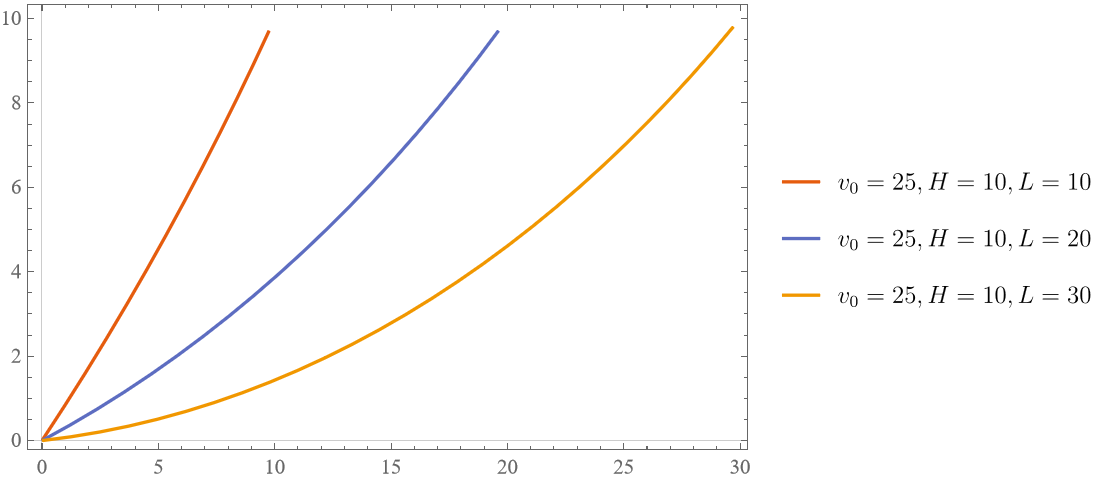
\includegraphics[width=10cm]{figure/fastest-ascedning.png}
\end{center}

\paragraph*{水平初速度约束}
\begin{example}
无约束最速升线的基础上,限定初速度与$x$轴平等,再次求解。
\end{example}
\begin{solution}

\end{solution}
\subsubsection{连续问题的一阶欧拉拉格朗日方程}
给定单变量函数优化问题

\begin{empheq}[left=\empheqlbrace]{align*}
\min_{\bm{q}}&\int_{t_0}^{t_1}L(\bm{q}(t),\bm{q}'(t),t)\\
\bm{q}(t_0)&=\bm{a}\\
\bm{q}(t_1)&=\bm{b}\\
\bm{q}&\colon \mathbb{R}\rightarrow \mathbb{R}^K
\end{empheq}

它等价于下面的欧拉-拉格朗日方程:
$$\frac{\dif }{\dif t}L_{\bm{q}_j'}(\bm{q},\bm{q}',t)-L_{\bm{q}_j'}(\bm{q},\bm{q}',t)=0,j=1\cdots,K$$

跟凸优化类似.注意,仅求解方程实际上并不能一定说解就是最小化原问题的解.更确切地说是求得驻点或者是潜在的稳态解.另外对$L$求导时,我们把$\bm{q}'$当作变量,并非链式法则.

多变量时,结果类似.问题

\begin{empheq}[left=\empheqlbrace]{align*}
	\min_{\bm{q}}&\int_{t_0}^{t_1}L(\bm{q},\partial \bm{q},\bm{x})\dif \bx\\
	\bm{q}&=\bm{\phi},\text{在}\partial D\text{上}\\
	\bm{q}&\colon \mathbb{R}^N\rightarrow \mathbb{R}^K
\end{empheq}

欧拉-拉格朗日方程为
$$\sum_{k=1}^n \partial_j L_{\partial_j \bm{q}_k}-L_{\bm{q}_k}=0,k=1,\cdots,K$$

注意这里是求和,单变量问题中只有一个变量,就没有求和.
